\documentclass[12pt, openany]{report}
\usepackage[utf8]{inputenc}
\usepackage[T1]{fontenc}
\usepackage[a4paper,left=2cm,right=2cm,top=2cm,bottom=2cm]{geometry}
\usepackage[frenchb]{babel}
\usepackage{libertine}
\usepackage[pdftex]{graphicx}

\setlength{\parindent}{0cm}
\setlength{\parskip}{1ex plus 0.5ex minus 0.2ex}
\newcommand{\hsp}{\hspace{20pt}}
\newcommand{\HRule}{\rule{\linewidth}{0.5mm}}

\begin{document}

\begin{titlepage}
  \begin{sffamily}
 \begin{center}

     % Upper part of the page. The '~' is needed because \\
     
\includegraphics[height=1.5cm,width=1.5cm]{1.PNG} \hspace{8.5cm}
     
\includegraphics[height=1.5cm,width=1.5cm]{2.PNG} \\

        \textsc{\ Université Cheikh Anta Diop \\Faculté Des Sciences Et Techniques\\Laboratoire Algèbre Cryptographie Géométrie Algébrique Application}\\[1.5cm]





     % Title
      \HRule \\[0.4cm]
          { \huge \bfseries Mise en place d'une application WEB pour la gestion d'un e-parking\\[0.4cm] }
       \HRule \\[0.2cm]


     % Author and supervisor
    \begin{minipage}{0.4\textwidth}
      \begin{flushleft} \large
        \emph{Président du jury :}
               \\ \textsc{Pr. Mamadou BARRY}\\
      \emph{Membres du jury :}
     

      \end{flushleft}
       \hspace{10.5cm}
    \end{minipage}
    \begin{minipage}{0.4\textwidth}
      \begin{flushright} \large
       \emph{Soutenu par :}
         \\ \textsc{Aminata DIALLO
         \newline
         Thierno Mamoudou Sabaly 
              }\\
   \emph{Sous la direction de :}
   \\ Mr. \textsc{Habib NDIAYE}\\



      \end{flushright}
    \end{minipage}

    \vfill

    % Bottom of the page
    {\large {}Année académique :2017-2018}

  \end{center}
  \end{sffamily}
\end{titlepage}
\newpage
   \thispagestyle{empty}
   \newpage

\newpage
   \thispagestyle{empty}

  \vfill




  \vfill

\newpage

   \begin{center}
    \LARGE
       \underline{\textsc{Remerciements}}
    \end{center}



    \LARGE

   \textbf{
   \textsc{
En préambule à ce mémoire je remercie notre créateur Allah pour tous ses bienfaits. Je voudrais exprimer ma gratitude à toute ma famille qui m'a soutenue, encouragée et assistée, plus particulièrement à mes parents. Puis, j'adresse mes sincères remerciements à mon encadreur Mr Habib NDIAYE pour m'avoir guidée, orientée, conseillée, critiquée afin de toujours donner le meilleur de moi-même. Mais aussi d'avoir cru en moi. Enfin, je remercie mes amis pour leurs soutiens inconditionnels et leurs encouragements. Ainsi que tous ceux qui de loin ou de près ont contribué à la réalisation de ce projet. À tous ces intervenants, je présente mes remerciements, mon respect et ma gratitude pour avoir fait de moi ce que je suis.}
 }



   \vfill
    \vfill
        \newpage
           \thispagestyle{empty}
           \begin{center}
                 \LARGE
               \textsc{   \underline{Dédicaces}}
                  \end{center}
                   \begin{center}

                      \LARGE
\begin{description}
\textbf{
\textsc{
Je voudrais dédier ce mémoire à toutes les personnes qui me sont chères. Mais aussi à tous les passionnés de "l'Internet of Thing"(IOT). Ces gens qui, nuit et jour, m'ont soutenue et ont cru en moi. À tous ceux qui liront ce mémoire, je vous souhaite de tout cœur que la lecture de ce mémoire soit une aubaine ou source d'inspiration pour vous.}}
\end{description}



               \vfill
               \begin{flushright}
               AMINATA  DIALLO
               \newline
               Thierno Mamoudou Sabaly
               \end{flushright}

                      \end{center}
           \vfill
      \newpage

   \large
   \tableofcontents
   \large
   \listoffigures
    \large
     \listoftables

      \vfill
   \newpage
      \thispagestyle{empty}

   \vfill

   \chapter{Introduction}

L'authentification automatique des individus devient une approche primordiale dans le monde, plus particulièrement dans le domaine de la sécurité et du contrôle des accès. D'une part, l'importance des enjeux motive les fraudeurs à mettre en échec les systèmes de sécurité existants.
\newline
Dans un tel cadre, la gestion de la sécurité constitue un véritable problème.
Il existe un intérêt grandissant pour les systèmes électroniques. Dès lors, comment assurer la gestion de la sécurité?
\newline
En ce sens, nous allons étudier les objectifs de ce système de sécurité basé sur une double authentification, puis expliquer le fonctionnement de chaque composant de ce dernier et enfin procéder à la réalisation de ce système.

        \newpage
         \thispagestyle{empty}
     \chapter{Étude de cas}
     \large
Le principe de notre système de sécurité repose sur le contrôle des accès. Lorsque l'individu veut accéder à un local, il doit dans un premier temps s'identifier grâce à son empreinte digitale. L'empreinte digitale de l'individu sera comparée aux empreintes contenues dans la base de données. Si l'empreinte est reconnue dans la base de données, alors il devra entrer mot de passe. Ce mot de passe saisi sera comparé au mot de passe enregistré dans le système. Dès lors se présenteront deux cas à savoir:

         \begin{itemize}
\item Le mot de passe est correct, une led verte va clignoter et il pourra accéder au local.
\item Sinon le mot de passe n'est pas correct, il devra entrer à nouveau son mot de passe. Si le mot de passe est correct il pourra accéder au local. Après 3 tentatives incorrectes du mot de passe ou de l'empreinte, un système d'alarme sera déclenché.
         \end{itemize}


 \chapter{Approche expérimentale}


 \subsection{Définition du module Arduino}
 \large
Le module Arduino est un circuit imprimé en matériel libre(plateforme de contrôle) dont les plans de la carte elle-même sont publiés en
licence libre. Un microcontrôleur programmé peut analyser et produire des signaux électriques de manière à effectuer des tâches très
diverses. Arduino est utilisé dans beaucoup d'applications comme l'électrotechnique industrielle et embarquée, le modélisme, la domotique
mais aussi dans des domaines différents comme l'art contemporain et le pilotage d'un robot, commande des moteurs, faire des jeux de
lumière, communiquer avec l'ordinateur, commander des appareils mobiles (modélisme). Chaque module d'Arduino possède un régulateur de
tension +5V et un oscillateur à quartz de 16MHz(ou un résonateur céramique de certains modèles). Pour programmer cette carte, on utilise
le logiciel Arduino IDE.

\subsection {Les différentes gammes de la carte Arduino}
\newpage
\begin{table}[!h]


{\large }
\begin{tabular}{|p{1,5cm}|p{1,5cm}|p{2cm}|p{3cm}|p{2cm}|c|c||}
\hline Carte Arduino & nom  & taille & micro controleur &memoire flash  & EEPROM & Alimentation

 \\
\hline  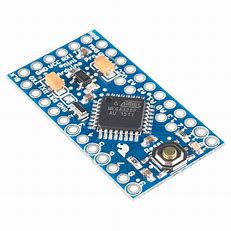
\includegraphics[height=1cm,width=1cm]{mini.jpg}& mini & 33x18x10   & ATmega328   & 32 (2) & 1  &7 – 9    \\
\hline  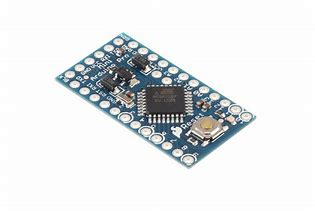
\includegraphics[height=1cm,width=1cm]{minipro.png}& mini PRO&  33x18x10
& Atmega168 & 16 (2) & 0.5 &
3.3-12 / 5-12   \\
\hline  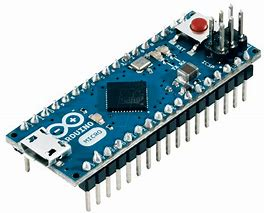
\includegraphics[height=1cm,width=1cm]{micro.jpg} & micro & 50x18x18 & Atmega32u4
& 32 (4) & 1 & 7 – 12 \\
\hline  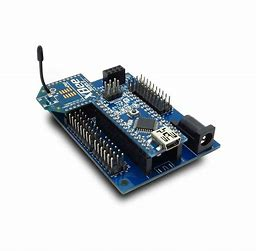
\includegraphics[height=1cm,width=1cm]{nano.jpg} & nano & 44x20x18 & Atmega168/328 & 16/32(2) &  0.5/1 & 7 – 12 \\
\hline  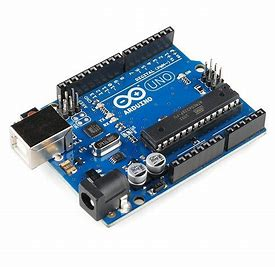
\includegraphics[height=1cm,width=1cm]{uno.png} & uno & 74x54x16 & Atmega328 & 32 (0.5) & 1
& 7 – 12   \\
\hline  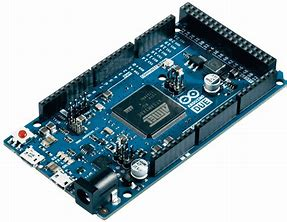
\includegraphics[height=1cm,width=1cm]{due.jpg} & due & 102x53x16 & AT91SAM3X8E & 512 &  &
7 – 12  \\
\hline  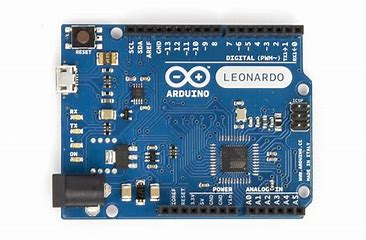
\includegraphics[height=1cm,width=1cm]{leonardo.png} & leonardo & 70x54x16 & Atmega32u4 & 32 (4)&
1 & 7 – 12 \\
\hline  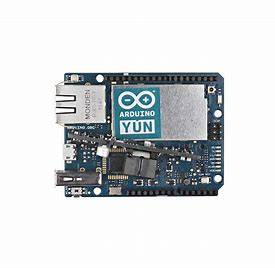
\includegraphics[height=1cm,width=1cm]{yun.png}  & Yun &  72x53x17 &
Atmega32u4,
 Atheros
  AR9331  &
32 (4) &
1 &
5  \\
\hline  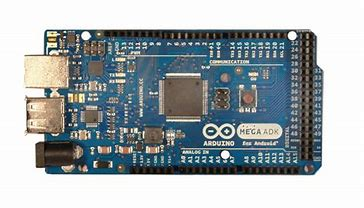
\includegraphics[height=1cm,width=1cm]{megaadk.jpg}& Mega ADK & 102x54x16 &
Atmega2560 &
256 (8) &
4 &
7 – 12  \\
\hline  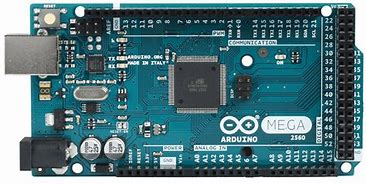
\includegraphics[height=1cm,width=1cm]{mega2560.jpg} & Mega 2560 &
107x53x15 &
Atmega2560 &
256 (8) &
4 &
7 – 12  \\

\hline  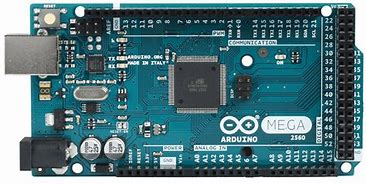
\includegraphics[height=1cm,width=1cm]{mega2560.jpg} &  Pro &
53x52x10 &
Atmega168/328 &
16/32 (2) &
0.5/1  &
3.3-12 / 5-12    \\
\hline  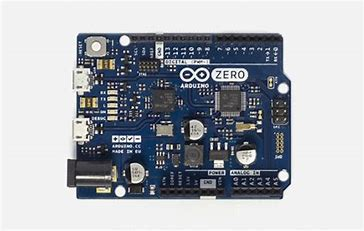
\includegraphics[height=1cm,width=1cm]{zero.jpg}& zero & &
ATSAMD21G18 &
256 &
16   \\
\hline  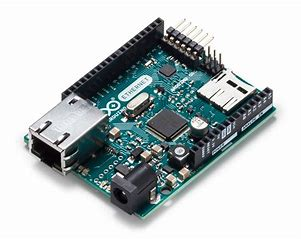
\includegraphics[height=1cm,width=1cm]{ethernet.jpg}& ethernet & &
ATmega328 &
32(0.5) &
1 &
7-12   \\
\hline
\end{tabular}
\newline

\caption{Tableau récapitulatif des différents types d'Arduino}
\end{table}         		          	
	
La mémoire EEPROM\footnote{Electrically-Erasable Programmable Read-Only Memory} est un type de mémoire morte. Une mémoire morte est un type de mémoire utilisée pour enregistrer des informations
 qui ne doivent pas être perdues lorsque l'appareil qui les contient n'est plus alimenté en électricité .        		          		
\subsection{ Le Micro contrôleur ATMega2560 }
Un microcontrôleur ATMega2560 est un circuit intégré, qui rassemble sur une puce plusieurs éléments complexes dans un espace réduit, au
temps des pionniers de l'électronique. Aujourd'hui, en soudant un grand nombre de composants encombrants tels que les transistors, les
résistances et les condensateurs, tous peuvent être logés dans un petit boîtier en plastique noir muni d'un certain nombre de broches
dont la programmation peut être réalisée en langage C. La figure suivante montre un microcontrôleur ATmega2560, qu'on trouve sur la carte
 Arduino.
\begin{figure}[!h]
    \centering
  
    \caption{Schéma des types de microcontrôleur} 		
\end{figure}
		
\subsection{Broches de connexion}
La carte Mega2560 dispose de 16 entrées analogiques, chacune pouvant fournir une mesure d'une résolution de 10 bits(c-à-d sur 1024 niveaux
 soit de 0 à 1023) à l'aide de la très utile fonction \textbf{analogRead()} du langage Arduino. Par défaut, ces broches mesurent entre
  le 0V(valeur 0) et le 5V(valeur 1023), mais il est possible de modifier la référence supérieure de la plage de mesure en utilisant la
broche AREF et l'instruction \textbf{analogReference()} du langage Arduino.
\underline{Note}: Les broches analogiques peuvent être utilisées en tant que broches numériques.
Il y a deux autres broches disponibles sur la carte :
\begin{enumerate}
    \item AREF: Tension de référence pour les entrées analogiques (si différent du 5V). Utilisée avec l'instruction analogReference().
    \item Reset: Mettre cette broche au niveau BAS entraîne la réinitialisation(le redémarrage) du micro-contrôleur. Typiquement, cette broche est utilisée pour ajouter un bouton de réinitialisation sur le circuit qui bloque celui présent sur la carte.
         		 \end{enumerate}
         		
         		 \subsection{Les ports de communications}
         		 La carte Arduino Mega2560 dispose de toute une série de facilités pour communiquer avec un ordinateur, une autre carte Arduino, ou avec d'autres microcontrôleurs. L'ATmega2560 dispose de quatre UARTs\footnote{Universal Asynchronous Receiver Transmitter}(émetteur-récepteur asynchrone universel en français) pour la communication série de niveau TTL(5V) et qui est disponible sur les broches 0(RX) et 1(TX). Un circuit intégré ATmega8U2 sur la carte assure la connexion entre cette communication série de l'un des ports série de l'ATmega 2560 vers le port USB de l'ordinateur qui apparaît comme un port COM virtuel pour les logiciels de l'ordinateur. Le code utilisé pour programmer l'ATmega8U2 utilise le driver standard USB COM, et aucun autre driver externe n'est nécessaire. Cependant, sous Windows, un fichier .inf est requis.
         		 Le logiciel Arduino inclut une fenêtre terminal série(ou moniteur série) sur l'ordinateur qui permet d'envoyer des textes simples depuis et vers la carte Arduino. Les LEDs RX et TX sur la carte clignotent lorsque les données sont transmises via le circuit intégré ATmega8U2 utilisé en convertisseur USB-vers-série et la connexion USB vers l'ordinateur(mais pas pour les communications série sur les broches 0 et 1).
         		 Une librairie Série Logicielle permet également la communication série(limitée cependant) sur n'importe quelle broche numérique de la carte UNO.
         		 L'ATmega2560 supporte également la communication par protocole I2C (ou interface TWI\footnote{Two Wire Interface}( Interface "2 fils") et SPI :
         		 \begin{enumerate}
         		 \item Le logiciel Arduino inclut la librairie Wire qui simplifie l'utilisation du bus I2C.\footnote{Voir la documentation pour les détails}
         		 \item Pour utiliser la communication SPI(Interface Série Périphérique), la librairie est disponible.
         		
         		 \end{enumerate}
         \begin{figure}[!h  ]
          \centering

  \caption{Schéma récapitulatif des différents ports de communication}
         		          		
 \end{figure}
 \newpage
         		
         		
         		 \section{Partie programme}
         		
         		 Une telle carte d'acquisition qui se base sur la construction d'un microcontrôleur doit être dotée d'une interface de programmation. L'environnement de programmation open-source pour Arduino peut être téléchargé
         		 gratuitement (pour Mac OS X, Windows, et Linux).
         		 \subsection{ Environnement de la programmation}
         		   \begin{figure}[!h]
         		                    \centering
         		 
         		             \caption{Structure générale du programme}
         		                   		          		
         		      \end{figure}
         		 Le logiciel de programmation de la carte Arduino sert d'éditeur de code(Langage
         		 proche du C). Une fois, le programme tapé ou modifié au clavier, il sera transféré et
         		 mémorisé dans la carte à travers de la liaison USB. Le câble USB alimente à la fois en énergie la carte et transporte aussi l'information.
         		 \subsection{Structure générale du programme (IDE Arduino)}
         		 Comme la plupart des langages de programmation, le code source est exécutable sur n'importe quel système d'exploitation basé sur la programmation
         		 en C. Les fonctions Setup et Loop sont obligatoires pour la création d'un programme en arduino .
         		 La fonction setup n'est exécutée qu'une seule fois, elle initialise et fixe les valeurs de démarrage du programme. La fonction Loop quant à elle s'exécute sans fin elle peut aussi permettre de contrôler la carte arduino
 
              		       		
         		
         		 \subsection{Injection du programme}
         		 Avant d'envoyer un programme dans la carte, il est nécessaire de sélectionner le type de la carte(Arduino UNO) et le numéro de port USB(COM3) comme à titre d'exemple cette
         		 figure suivante.
  \begin{figure}[!h]
                \centering

         \caption{Initialisation de la carte }
               		          		
               		          		 \end{figure}
           		       		
         		
         	\newpage	
         		
         		
         		 \subsection{Description du programme}
         		 Un programme arduino est une suite d'instructions élémentaires sous forme textuelle
         		 (ligne par ligne). La carte lit puis effectue les instructions les unes après les autres dans l'ordre défini par les lignes de code.
         		
         		 \textbf{Les commentaires}
         		 Les commentaires sont, en programmation informatique, des portions du code source ignorées par le compilateur ou l'interpréteur car ils ne sont pas censés influencer l'exécution
         		 du programme.
         		
         		 \textbf{Définition des variables}
         		 Pour notre montage, on va utiliser une sortie numerique de la carte qui est par exemple
         		 la 3e sortie numérique. Cette variable, doit étre définie et nommée ici buzzer pin 3; la
         		 syntaxe est pour désigner un nombre entier est int.
         		
         		 Une programmation des interactions void loop: dans cette boucle, on définit les opérations à effectuer dans l'ordre digital write nom, état) est une autre des quatre fonctions relatives aux entrées – sorties numériques.
         		
         		 delay(temps en mili-seconde) est la commande d'attente entre deux instructions.
         		
         		 chaque ligne d'instruction est terminée par un point-virgule. Ne pas oublier les accolades qui encadrent la boucle.
         		
         		
         		 void loop()
         		
         		
         		 { ---------------------------------------------------------------------------------------------
         		
         		
         		 10 digital write ( moteur 1,HIGH);
         		 ---------------------------------------------------------------------
         		
         		 11delay(3000)---------------------------------------------------------------------------------------------
         		
         		 12 digital Write(buzzer 1, LOW) ;
         		 -----------------------------------------------------------------------
         		
         		 13 delay
         		 \vspace{1cm} (1000)---------------------------------------------------------------------------------------------
         		
         		 14 }-----------------------------------------------------
         		
         		 \subsection{Les étapes de téléchargement du programme }
         		 1. On conçoit ou on ouvre un programme existant avec le logiciel IDE Arduino.
         		
         		 2. On vérifie ce programme avec le logiciel Arduino(compilation).
         		
         		 3. Si des erreurs sont signalées, on modifie le programme.
         		
         		 4. On téléverse le programme sur la carte.
         		
         		 5. On câble le montage électronique.
         		
         		 6. L'exécution du programme est automatique après quelques secondes.
         		
         		 7. On alimente la carte soit par le port USB, soit par une source d'alimentation autonome
         		 (pile 9 volts par exemple).
         		
         		 8. On vérifie que notre montage fonctionne.
      \begin{figure}[!h]
                     \centering
     
              \caption{Initialisation de la carte }
                    		          		
                    		          		 \end{figure}
                \newpage		       		 		
         		
        \section{Les différents composants de notre système}
  La carte Arduino est généralement associée aux accessoires qui simplifient les réalisations.
 \subsection{ Les afficheurs LCD}
  Les écrans LCD existent depuis 1971. Ils n'ont pas cessé de se développer depuis, et équipent maintenant bien des appareils à affichage embarqué(appareils photo, digicodes, montres, téléphones). LCD est l'abréviation anglaise de “liquid crystal display” qui veut dire : afficheur à cristaux liquides. Cette technologie permet de créer des écrans plats qui consomment peu d'énergie. Parmi les écrans lcd nous pouvons citer l'afficheur I2C, les afficheur 1*16, 20*4, le shield keypad LCD, etc... Nous nous intéresserons à l'écran LCD 16*2. L'écran LCD 16*2 nous permettra d'afficher les données saisies par l'utilisateur.
 \begin{figure}[!h]
                \centering
 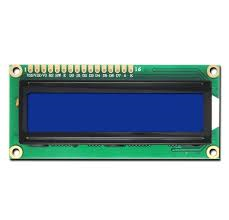
\includegraphics[height=10cm,width=10cm]{lcd.png} 
         \caption{Schéma de l'écran LCD }
               		          		
               		          		 \end{figure}
                		 
 \begin{figure}[!h]
                 \centering
 \subsection{RFID}
 RFID, qui signifie identification par radio fréquence, est une méthode permettant de récupérer et traiter des données à distance. Le système est activité par un transfert d’énergie électromagnétique entre une étiquette radio et un émetteur RFID. L' Étiquette radio, appelée tag, est composée d’ une puce électronique et d’une antenne qui reçoit le signal emis par le lecteur équipé d’ une technologie RFID. Les composantes permettent delire et répondre aux signaux
  La RFID est caractérisé par la Fréquence. Celle-ci permet d’établir la communication entre la puce et l’antenne.Il existe ainsi différentes puce,leur différence régide sur la fréquence de fonctionnement et la distance de lecture. Plus la fréquence est élevée, plus la distance de lecture s’agrandi. Trois types de fréquence sont utilisées par les puce RFID : Basse fréquence (125KHZ), Haute fréquence (13,56MHZ) et Très haute fréquence(UHF):
  \begin{enumerate}
  \item  RFID passive : C ’ est un ensemble de puce fonctionnant en lecture seule. N ’ ayant pas de batterie, elles se déplacent vers les lecteurs pour être activé par un signal électromagnétique.Cet alimentation permettra la lecture des données qu ’ il contient
  \item  RFID active : Contrairement à la précédente, cette technologie permet une lecture à longue distance des puces. Et ceci,grâce à la source d’ énergie(pile ou batterie)qu ’ utilise ces puces. 
  \item  RFID semi-passive : ça serait une sorte d’ intermédiaire évidemment, ces puce possède des sources d’ énergies mais qui leur alimente que par intervalle de temps.
  
  \end{enumerate} 
 
 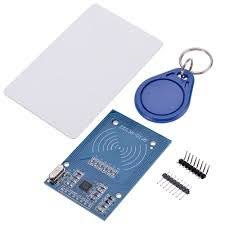
\includegraphics[height=5cm,width=5cm]{rfid.png} 
          \caption{Schéma du clavier Matricielle keypad}
               		          		
 \end{figure}

          \newpage      	
   \subsection{ Buzzer}
   Les buzzer sont des périphériques qui nous permette d'émettre un signal sonore à partir de tonalité. Il existe deux types de buzzer à savoir le buzzer actif et le buzzer passif.	  		         							    Un buzzer actif va générer une tonalité à l'aide d'un oscillateur interne de sorte que tout ce qui est nécessaire est une tension CC. Un buzzer passif nécessite un signal ca pour faire un son. C'est comme un haut-parleur électromagnétique où un signal d'entrée changeant, plutôt que de produire une tonalité automatiquement.
   La méthode pour les identifier est la suivante: si vous appliquez une tension CC il vibre, alors nous avons un buzzer actif sinon un buzzer passif.
   En ce qui concerne les commandes nous allons contrôler le pitch. PWM sur l'Arduino peut être utilisé pour contrôler le pitch et le volume en même temps(qui peut ou peut ne pas être ce que vous voulez). Si nous voulons changer juste levolume ou juste le pitch je suppose que certains circuits externes seraient nécessaires pour changer l'amplitude sans changer la tension, et vice versa. Ainsi ce buzzer va nous fournir la tonalité nécessaire afin de déclencher l'alarme.
  \begin{figure}[!h]
                  \centering
 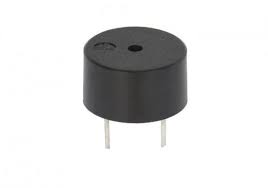
\includegraphics[height=5cm,width=5cm]{buzzer.jpg} 
           \caption{Schéma du buzzer actif}
                 		          		
  \end{figure}  		         				    	\subsection{Servo moteur}	
  Un servomoteur de modélisme se présente sous la forme d ’ un petit rectangle avec deux languettes sur les côtés pour la fixation et un axe décentré avec un bras(interchangeable) pour la liaison mécanique. Le servomoteur est un moteur esclave. Esclave parce que l ’ on lui ordonne et il obéit. On peut
  remarquer de petit gros servomoteurs,ils sont essentiellement constitués d’ une boite, d’ un axe et d ’ une roue (ou barre) trouée. Il y ’ a des servomoteur hydrauliques, mais nous utiliserons de ceux électriques dans le cadre de ce projet. Un servomoteur est constitué d’ un moteur à courant continu. Il tourne lorsqu'il parcouru par de l’ électricité. Ce moteur est associé à une série d ’ engrenages. Une série d ’ engrenage est un ensemble de roue dentées qui s ’ entrainent les unes des autres lors de leur rotation,on par le de train d ’ engrenage. Ce train met en rotation l ’ axe apparent à l ’ extérieur du moteur. Un servomoteur est caractérisé par un couple (kg.cm) exprimant la masse qu ’ il peut entrainer à une certaine distance de son axe. Ce couple est définit comme étant la force nécessaire pour faire tourner l ’ axe.
     \begin{figure}[!h]
                     \centering
    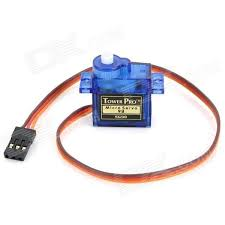
\includegraphics[height=5cm,width=5cm]{servomoteur.jpg} 
              \caption{Schéma du servomoteur}
                    		          		
     \end{figure}    									\subsection{Capteur d'ultra-sons}
     	
      \begin{figure}[!h]
                          \centering
         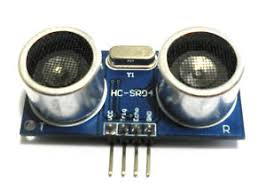
\includegraphics[height=5cm,width=5cm]{ultrasons.png} 
                   \caption{Schéma du capteur d'ultrasons}
                         		          		
          \end{figure}
    \subsection{ capteur d'infrarouge}
           \begin{figure}[!h]
                                    \centering
                   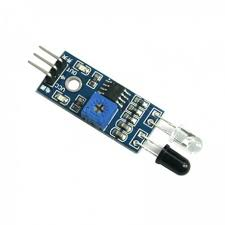
\includegraphics[height=5cm,width=5cm]{infrarouge.png} 
                             \caption{Schéma du capteur  d'infrarouge}
                                   		          		
                    \end{figure} 	
\end{document} 